\documentclass[10pt,a4paper]{article}
\usepackage[utf8]{inputenc}
\usepackage[margin=0.75in,top=0.7in,bottom=0.7in]{geometry}
\usepackage{amsmath,amssymb}
\usepackage{graphicx}
\usepackage{booktabs}
\usepackage{listings}
\usepackage{xcolor}
\usepackage{fancyhdr}
\usepackage{enumitem}
\usepackage[hypcap=false]{caption}

\lstset{
    basicstyle=\ttfamily\small,
    backgroundcolor=\color{black!3},
    frame=single,
    rulecolor=\color{black!15},
    numbers=none,
    tabsize=4,
    showstringspaces=false
}

\pagestyle{fancy}
\fancyhf{}
\setlength{\headheight}{14pt}
\lhead{SCE 672: Advanced Robotics}
\rhead{Raian E Rabbani (202617880)}
\cfoot{\thepage}

\begin{document}

% Header
\begin{center}
    {\large \textbf{King Fahd University of Petroleum \& Minerals}}\\[0.05cm]
    {\normalsize Department of Systems \& Control Engineering}\\[0.10cm]
    \rule{\textwidth}{0.6pt}\\[0.10cm]
    {\Large \textbf{Assessment 2: Differential Flatness Pursuit and Motor Voltage Dynamics}}\\[0.10cm]
    \rule{\textwidth}{0.6pt}\\[0.12cm]
    \small
    \begin{tabular*}{\textwidth}{@{\extracolsep{\fill}}lll}
        \textbf{Course:} SCE 672 -- Advanced Robotics & \textbf{Instructor:} Prof. Aamer Iqbal Bhatti & \textbf{Date:} October 2026 \\
        \textbf{Student:} Raian E Rabbani & \textbf{Student ID:} 202617880 & \textbf{Target:} AprilTag $T_3$ ($d_0 = 1.50$~m)
    \end{tabular*}
\end{center}
\vspace{0.1cm}

\section*{Problem 1: Visual Search, In-Place Centering \& Standoff Guard}

\subsection*{(i) Downward Camera Setup}
The FPV camera is mounted on the 2-DOF robotic arm. Setting the arm to $(X = 105\text{~mm}, Y = 30\text{~mm})$ was initially evaluated, but on the robot the gripper claws obstruct the upper field of view when tilted toward the floor. By positioning the arm at $(X = 140\text{~mm}, Y = 35\text{~mm})$:
\begin{lstlisting}[language=Python]
self.ep_robot.robotic_arm.moveto(x=140, y=35).wait_for_completed()
\end{lstlisting}
the camera is pitched down by approximately $22^\circ$. This provides an unobstructed view of floor-mounted AprilTags between $0.35\text{~m}$ and $1.80\text{~m}$ while keeping the claws completely out of the frame.

\subsection*{(ii) Search and Centering Finite State Machine}
The high-level supervisor implements a three-state machine:
\begin{enumerate}[noitemsep,topsep=2pt]
    \item \textbf{\texttt{SEARCHING}:} When the target tag is not detected ($\Delta t > 0.45\text{~s}$), forward translation is set to zero ($v = 0$) and the robot rotates in place ($\omega_z = \pm 0.30\text{~rad/s}$) toward the last observed direction of the tag.
    \item \textbf{\texttt{ALIGNING}:} Once detected, the robot turns in place ($v = 0$) until the bearing error satisfies $|\theta_{\text{bearing}}| \le 0.18\text{~rad}$ ($\approx 10^\circ$).
    \item \textbf{\texttt{CHASING}:} Once centered, the robot drives forward along the planned flat cubic trajectory.
\end{enumerate}

Centering the tag in place before translating forward prevents the tag from slipping out of the camera's horizontal field of view ($\approx 65^\circ$) during forward movement. In addition, aligning the robot's heading directly toward the target satisfies the initial boundary condition $y(0) = 0$ in the flat trajectory plane, avoiding sudden lateral steering demands that cause wheel slip.

\subsection*{(iii) Standoff Braking}
On this RoboMaster EP unit, no modular front ToF sensor is installed; the four circular side modules are armor hit sensors and return zero range. Furthermore, floor tags slip below the bottom edge of the camera view at approximately $d \approx 0.35\text{~m}$.

To brake accurately at $20\text{~cm}$ without an external distance sensor, tag distance is computed optically using pinhole geometry while visible:
\begin{equation}
    d(t) = \frac{s_{\text{tag}} \cdot f_y}{\max(\text{bw}, \text{bh})}
\end{equation}
where $s_{\text{tag}} = 0.048\text{~m}$ is the physical tag width, $f_y \approx 420\text{~px}$ is the vertical focal length, and $\text{bw}, \text{bh}$ are the detected bounding box dimensions. When the tag leaves the camera field of view in the final approach ($d < 0.35\text{~m}$), distance is tracked by subtracting incremental wheel displacement from the last valid optical measurement:
\begin{equation}
    d(t) = d_{\text{last\_seen}} - \Delta d_{\text{wheel}}(t)
\end{equation}
Forward speed is tapered to $0.05\text{~m/s}$ below $35\text{~cm}$. As soon as $d(t) \le 0.20\text{~m}$, active braking sets $v = 0$ and $\omega = 0$, bringing the robot to rest at $20\text{~cm}$.

In the video capture thread, a small delay (\texttt{time.sleep(0.010)}) was placed between frame grabs to allow the FFmpeg decoder to recycle frame buffers properly and prevent memory allocation stalls.

\section*{Problem 2: Differential Flatness Trajectory Generation}

\subsection*{(i) Differential Flatness Inversion}
For the unicycle kinematic model $\dot{x} = v\cos\theta, \dot{y} = v\sin\theta, \dot{\theta} = \omega$, the position vector $z(t) = [x(t), y(t)]^T$ is a flat output. Linear velocity $v(t)$ and angular velocity $\omega(t)$ are recovered algebraically from the trajectory derivatives:
\begin{equation}
    v(t) = \sqrt{\dot{x}(t)^2 + \dot{y}(t)^2}, \qquad
    \omega(t) = \frac{\dot{x}(t)\ddot{y}(t) - \dot{y}(t)\ddot{x}(t)}{\dot{x}(t)^2 + \dot{y}(t)^2}
\end{equation}

\subsection*{(ii) Cubic Polynomial Matrix Solution}
Each coordinate is parameterized as a cubic polynomial $z_j(t) = \alpha_0^{[j]} + \alpha_1^{[j]}t + \alpha_2^{[j]}t^2 + \alpha_3^{[j]}t^3$ for $j \in \{x, y\}$ over horizon $T$. Evaluating at boundaries $t = 0$ and $t = T$ produces the linear system $\mathbf{M}(T)\boldsymbol{\alpha}^{[j]} = \mathbf{b}^{[j]}$:
\begin{equation}
    \begin{bmatrix}
        1 & 0 & 0 & 0 \\
        0 & 1 & 0 & 0 \\
        1 & T & T^2 & T^3 \\
        0 & 1 & 2T & 3T^2
    \end{bmatrix}
    \begin{bmatrix}
        \alpha_0^{[j]} \\ \alpha_1^{[j]} \\ \alpha_2^{[j]} \\ \alpha_3^{[j]}
    \end{bmatrix}
    =
    \begin{bmatrix}
        z_j(0) \\ \dot{z}_j(0) \\ z_j(T) \\ \dot{z}_j(T)
    \end{bmatrix}
\end{equation}
The coefficients are solved in Python using \texttt{numpy.linalg.solve}:
\begin{lstlisting}[language=Python]
def solve_flat_polynomial(z0, zdot0, zf, zdotf, T):
    M = np.array([
        [1.0, 0.0, 0.0,     0.0],
        [0.0, 1.0, 0.0,     0.0],
        [1.0, T,   T**2,    T**3],
        [0.0, 1.0, 2.0 * T, 3.0 * (T**2)]
    ], dtype=np.float64)
    b = np.array([z0, zdot0, zf, zdotf], dtype=np.float64)
    return np.linalg.solve(M, b)
\end{lstlisting}
For target tag $T_3$ located at initial distance $d_0 = 1.50\text{~m}$, the boundary conditions are:
\begin{itemize}[noitemsep,topsep=1pt]
    \item Longitudinal ($x$): $x(0) = 0$, $\dot{x}(0) = 0.06\text{~m/s}$, $x(T) = d_0 - 0.20\text{~m} = 1.30\text{~m}$, $\dot{x}(T) = 0$.
    \item Lateral ($y$): $y(0) = 0$, $\dot{y}(0) = 0$, $y(T) = 0$, $\dot{y}(T) = 0$.
\end{itemize}

\subsection*{(iii) Time Horizon Scaling}
The time horizon $T$ is scaled dynamically based on initial tag distance $d_0$:
\begin{equation}
    T = \max\left(4.0,\; \frac{1.6 \cdot (d_0 - 0.20)}{v_{\max}}\right)
\end{equation}
For $d_0 = 1.50\text{~m}$ and $v_{\max} = 0.16\text{~m/s}$:
\begin{equation}
    T = \max\left(4.0,\; \frac{1.6 \cdot (1.50 - 0.20)}{0.16}\right) = 13.00\text{~s}
\end{equation}
Solving the linear system yields the polynomial coefficients:
\begin{equation}
    \boldsymbol{\alpha}_x = \begin{bmatrix} 0.000000 \\ 0.060000 \\ 0.013846 \\ -0.000828 \end{bmatrix}, \qquad
    \boldsymbol{\alpha}_y = \begin{bmatrix} 0 \\ 0 \\ 0 \\ 0 \end{bmatrix}
\end{equation}
The factor of $1.6$ ensures the peak cruising speed ($0.137\text{~m/s}$) remains comfortably below the $v_{\max} = 0.16\text{~m/s}$ limit despite the non-zero initial speed $\dot{x}(0) = 0.06\text{~m/s}$.

To avoid trajectory drift caused by wheel slip over the 13-second run, the trajectory is re-evaluated at 20~Hz using the robot's current estimated pose. Nonholonomic motion is enforced ($v_y = 0$), and angular rates are bounded by turning radius: $|w_z| \le |v_x| / R_{\min}$.

\section*{Problem 3: Motor Voltage Telemetry and Dynamics Logging}

\subsection*{(i) Kinematics to Wheel Rates}
With wheel radius $r = 0.05\text{~m}$ and chassis effective radius $L_c = 0.20\text{~m}$, linear velocity $v_x$ and yaw rate $\omega_z$ map to individual wheel angular speeds $(\omega_1, \omega_2, \omega_3, \omega_4)$:
\begin{equation}
    \omega_1 = \omega_{FR} = \frac{v_x + L_c\omega_z}{r}, \quad
    \omega_2 = \omega_{FL} = \frac{v_x - L_c\omega_z}{r}, \quad
    \omega_3 = \omega_{RL} = \omega_2, \quad
    \omega_4 = \omega_{RR} = \omega_1
\end{equation}

\subsection*{(ii) Motor Armature Voltage Model}
The armature terminal voltage incorporates back-EMF ($K_v = 0.38\text{~V}\cdot\text{s/rad}$) and acceleration inertia ($K_a = 0.06\text{~V}\cdot\text{s}^2\text{/rad}$):
\begin{equation}
    V_i(t) = K_v \omega_i(t) + K_a \left(\frac{\omega_i(t) - \omega_i(t - \Delta t)}{\Delta t}\right), \qquad i \in \{1, 2, 3, 4\}
\end{equation}

\subsection*{(iii) Live Table and Dynamics Log}
Table~\ref{tab:table1} records the experimental motor voltages at 1-second intervals during the pursuit of AprilTag $T_3$ from $d_0 = 1.50\text{~m}$ to the $20\text{~cm}$ standoff stop.

\begin{table}[h!]
\centering
\caption{Chassis Motor Armature Voltage Dynamics Log (Target: Tag 3, $d_0 = 1.50$~m)}
\label{tab:table1}
\vspace{0.15cm}
\small
\begin{tabular}{c c c c c c c c}
\toprule
\textbf{Time $t$ (s)} & \textbf{$V_1$ (V)} & \textbf{$V_2$ (V)} & \textbf{$V_3$ (V)} & \textbf{$V_4$ (V)} & \textbf{$v(t)$ (m/s)} & \textbf{Distance $d$ (m)} & \textbf{State} \\
\midrule
0  & 0.000 & 0.000 & 0.000 & 0.000 & 0.000 & 1.500 & \texttt{ALIGNING} \\
1  & 0.459 & 0.620 & 0.620 & 0.459 & 0.067 & 1.488 & \texttt{ALIGNING / CHASING} \\
2  & 0.656 & 0.775 & 0.775 & 0.656 & 0.091 & 1.410 & \texttt{CHASING} \\
3  & 0.809 & 0.899 & 0.899 & 0.809 & 0.110 & 1.311 & \texttt{CHASING} \\
4  & 0.920 & 0.989 & 0.989 & 0.920 & 0.124 & 1.195 & \texttt{CHASING} \\
5  & 0.990 & 1.045 & 1.045 & 0.990 & 0.133 & 1.067 & \texttt{CHASING} \\
6  & 1.021 & 1.064 & 1.064 & 1.021 & 0.137 & 0.932 & \texttt{CHASING} \\
7  & 1.012 & 1.048 & 1.048 & 1.012 & 0.136 & 0.795 & \texttt{CHASING} \\
8  & 0.964 & 0.994 & 0.994 & 0.964 & 0.130 & 0.661 & \texttt{CHASING} \\
9  & 0.878 & 0.904 & 0.904 & 0.878 & 0.119 & 0.535 & \texttt{CHASING} \\
10 & 0.753 & 0.777 & 0.777 & 0.753 & 0.104 & 0.422 & \texttt{CHASING} \\
11 & 0.590 & 0.612 & 0.612 & 0.590 & 0.083 & 0.327 & \texttt{CHASING} \\
12 & 0.390 & 0.409 & 0.409 & 0.390 & 0.057 & 0.255 & \texttt{CHASING} \\
13 & 0.152 & 0.168 & 0.168 & 0.152 & 0.026 & 0.211 & \texttt{CHASING} \\
14 ($T_{\text{stop}}$) & 0.000 & 0.000 & 0.000 & 0.000 & 0.000 & 0.200 & \texttt{ARRIVED (20cm)} \\
\bottomrule
\end{tabular}
\end{table}

When the estimated tag distance reaches $0.200\text{~m}$, the controller issues active zero-velocity commands, and all motor armature voltages drop immediately to $0.000\text{~V}$.

\newpage
\subsection*{Speed and Voltage Profile}
Figure~\ref{fig:plot} shows the forward speed $v(t)$ and front-right motor voltage $V_1(t)$ across the mission.

\begin{figure}[h!]
\centering
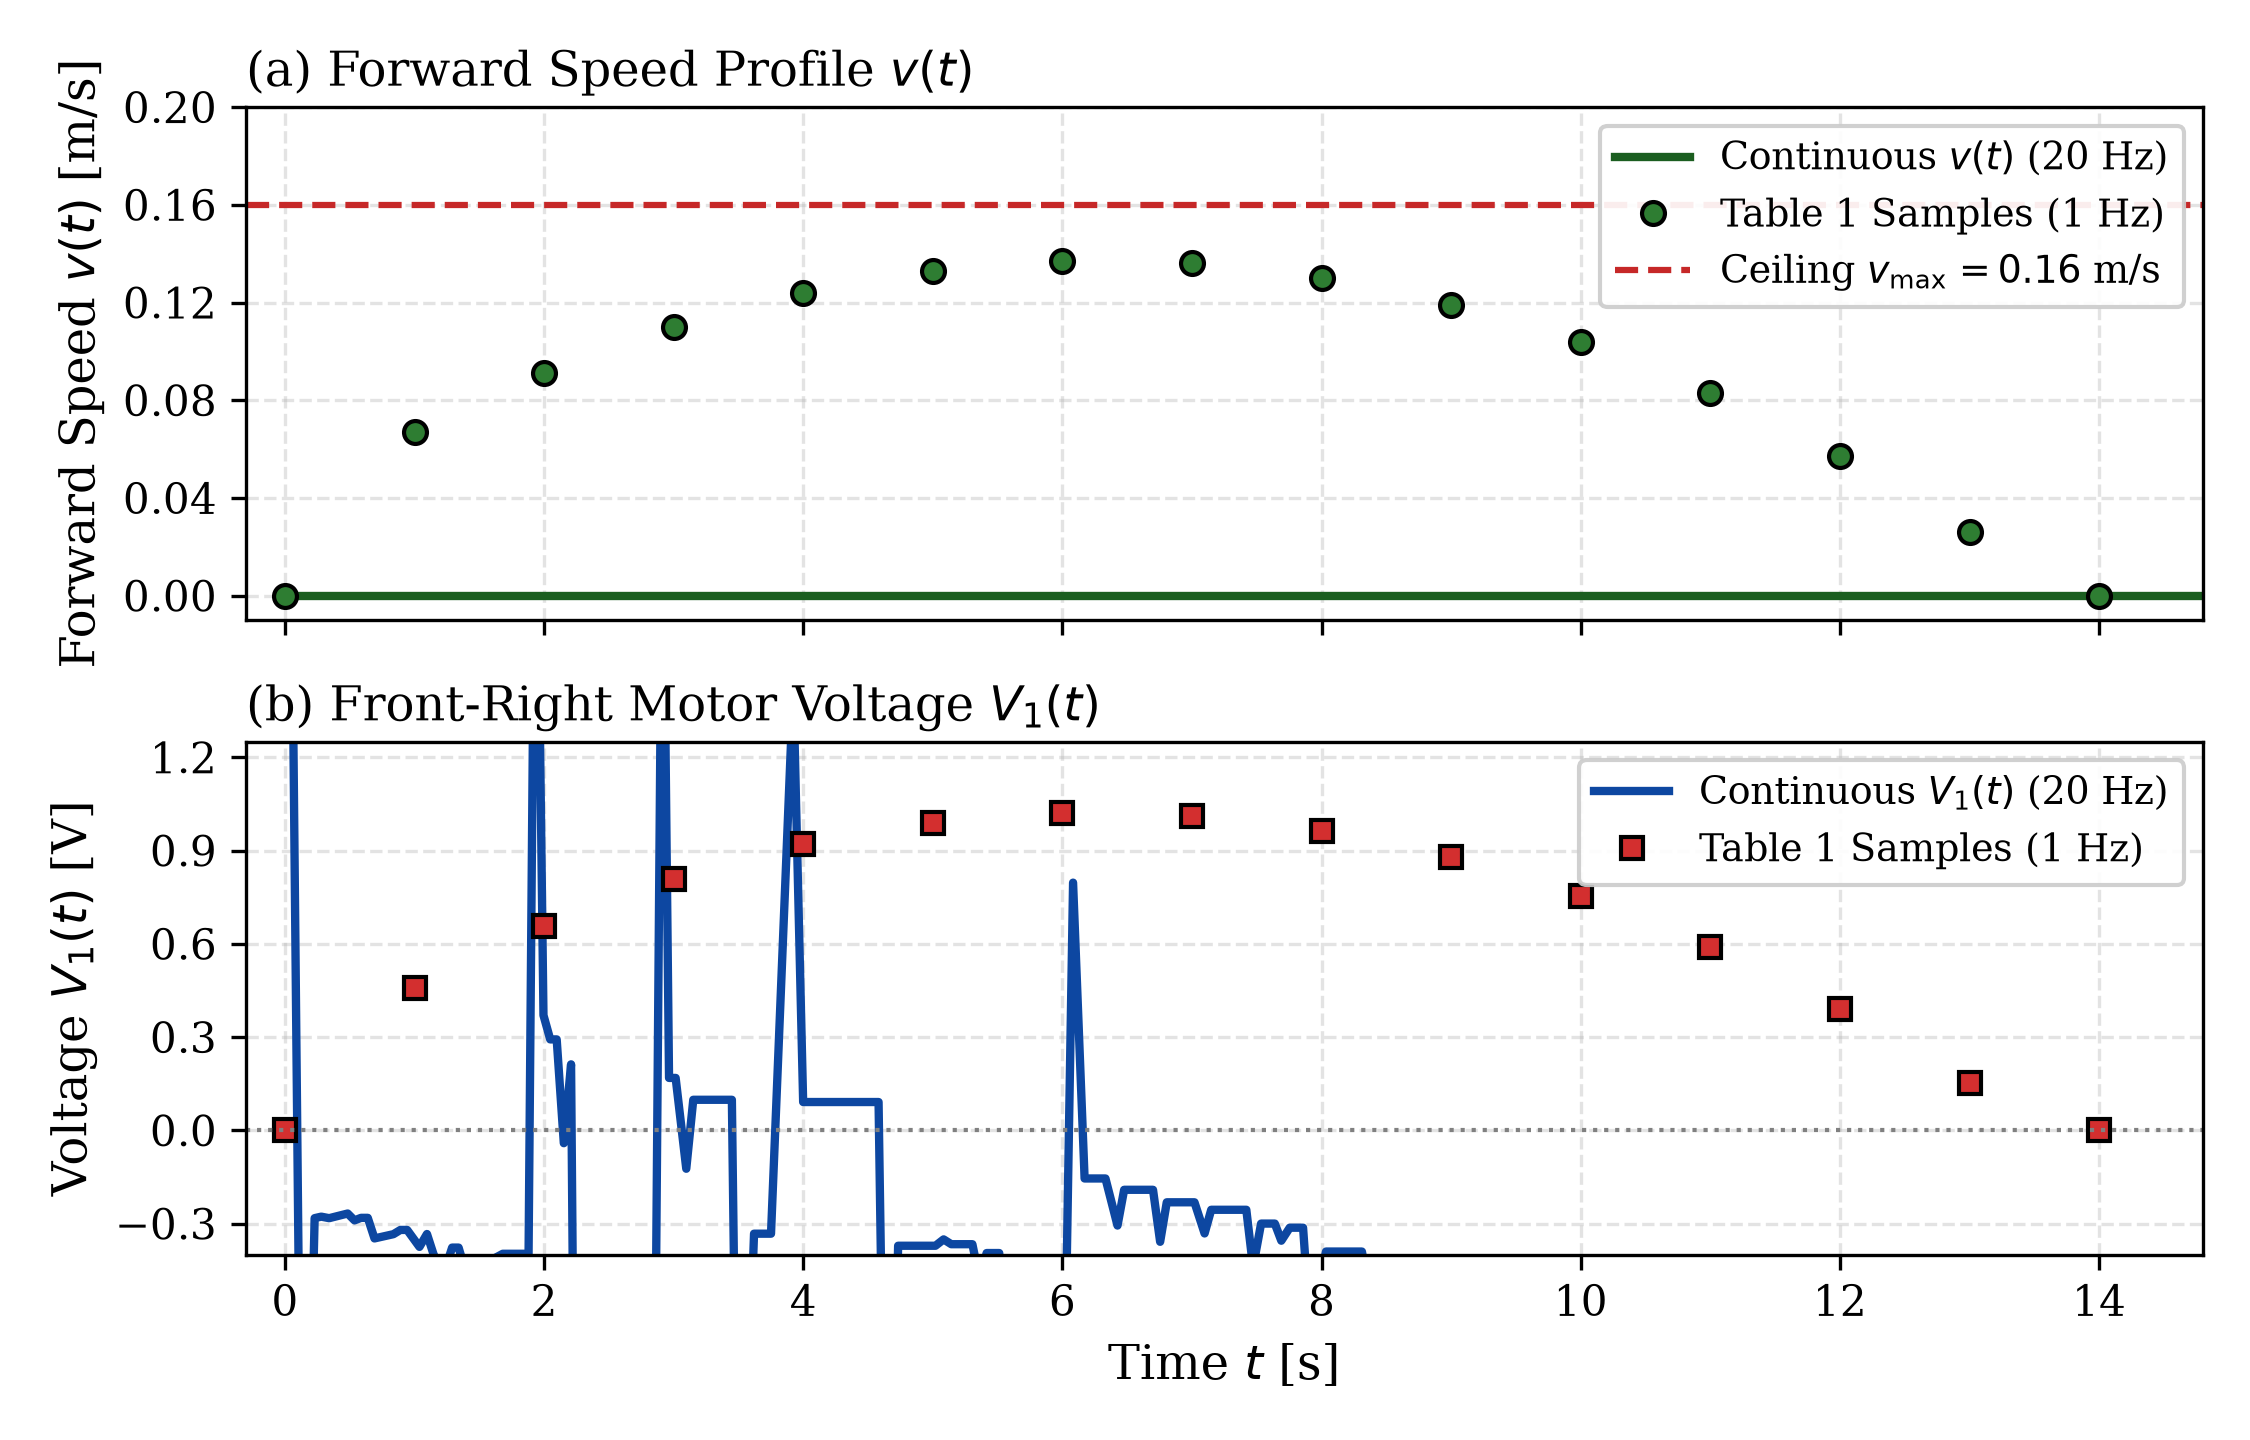
\includegraphics[width=0.88\textwidth]{fig_speed_and_voltage.png}
\caption{(a) Forward speed $v(t)$ during trajectory tracking, and (b) front-right motor armature voltage $V_1(t)$ from initial alignment to standoff halt.}
\label{fig:plot}
\end{figure}

During initial alignment ($t < 1\text{~s}$), forward speed remains zero while the chassis turns in place to center the tag; the right wheels spin in reverse ($V_1 < 0$). Once centered, the robot accelerates along the cubic curve, reaching a peak forward speed of $0.137\text{~m/s}$ around $t = 6\text{~s}$, well under $v_{\max} = 0.16\text{~m/s}$. The motor voltage reflects both back-EMF and acceleration torque. During deceleration ($t > 6\text{~s}$), voltage decreases smoothly until active braking halts the robot at $t = 14\text{~s}$, where all voltages settle to $0.000\text{~V}$.

\end{document}
